
Coirón is the computer system that manages the administration of cases admitted to the Public Prosecutor's Office of Chubut. 
It is a tool that allows the registration, communication and management of activities, procedures and actions that are carried out for a criminal case, from the initial charge to its final completion.
As a registration tool, it builds a database with the history of every case, as well as the people involved and those responsible for management in each office. 
As a communication tool, it groups information, allows cross-examination of relations, identifies links between cases, people, and their backgrounds. 
As a management tool, it manages the evolution of cases and the corresponding work of the officials. 
It allows planning, organizing, coordinating and controlling the workflow related to each case.
It has been developed according to the needs of the Public Prosecutor's Office of Chubut, based on the current Criminal Procedure Code and adapted to the strategic guidelines for the design and management of state Prosecutor's Offices defined by the federal Attorney General. 
Its progress, maintenance and continuous improvement is in charge of the Development Team of the Department of Information Technology of the Area of Planning and Management Control of the General Procurement.

Since Coirón is a software tool to support criminal investigation, it is important to enhance its features towards a smart provision of data.
In particular, we are interested in the analysis of criminal records in order to facilitate the identification of gangs. 
This should be paired with correct information visualization tools, enhancing the analysis that will be carried out later by criminal analysts.
In this paper we focus then on criminal gangs, applying techniques to acknowledge the \textit{relative importance} of their members, which can be visualized properly in a graph denoting social connections.
%Once all the information related to a fact is registered, and with the help of tools and links with other systems, outputs can be obtained that allow the investigation of a case or a set of facts with common characteristics to be carried out.
%We are incorporate information visualization tools that allow us to see in graphic mode what is currently displayed in grids and lists, enhancing the analysis that specialists will carry out later. 
A relational profile can be build for criminal prosecution, through the identification of "criminal partners" via the social network induced by criminal records, in order to identify if they are part of a simple street gang or some larger criminal organization~\cite{rua2020perspectiva}. 
Social network is represented as graphs, which are of great visual aid when working with a large number of records.
There are many variations on the graphs, but they all share the common feature of using a labeled circle for each actor in the population and line segments between pairs of actors to represent the fact that there is a link between them. 
The "\textit{Group of Membership}" in the \texttt{Coirón} system refers to the direct relationship between an individual within the universe of people charged as perpetrators of crimes (either involved, indicted or sentenced) and other individuals of the same universe, with one or more criminal cases in common.

A software module "Membership Group Network" graphically displays this data, enriched with information obtained by social network analysis. 
Through various filters, it is possible to graphically show the relationships between a certain group of people in order to identify the formation of possible criminal gangs.
%The central idea is to graphically reflect, by means of a Graph, the membership groups.
In the graph a node a person involved in two or more criminal cases.
There is a large number of people in the system with only one case with the role of \textit{reported}, and for this reason they are excluded. 
However they could be part of the dataset to be displayed if any of them are found related to other nodes of the first group. 
The size of the node is directly related to the number of criminal cases in which the person is involved. The larger the size of the node, the more criminal cases it will be involved in.

Line segments between pairs of nodes link people together and represent the case(s) they have in common. The thickness of the link will be directly proportional to the number of cases in common between a pair of people. There are nodes that will be isolated in the graph, this does not mean that they are not involved in cases, but that there may not be relationships for the search filter that is used in that particular view.
%Los segmentos de líneas entre pares de nodos, vinculan a las personas entre sí y representan el o los casos que tienen en común. El grosor de la vinculación será directamente proporcional a la cantidad de casos en común entre un par de personas. Hay nodos que se encontrarán aislados en el grafo, esto no significa que no estén involucrados en casos, sino que quizás no existan relaciones para el filtro de búsqueda que se utilice en esa vista en particular.

Suppose that a person "A" is associated with 8 criminal cases, a person "B" with 4 and a person "C" with 2 cases. Let's add that people "A" and "B" are related to each other, because they are in 3 cases in common (cases 1, 2 and 3). On the other hand, people "A" and "C" are also related, because they have a case in common (case 4). A graphical representation of this situation is shown in Figure \ref{fig:grafode2}, and the double size can be observed between node "A" and node "B", precisely representing the difference in cases between both nodes (8 and 4 cases). Also seen with the naked eye is the thickness of the link between "A" and "B" three times greater than the link between "A" and "C" (3 cases in common between the first pair of nodes, and only one case for the last mentioned pair of nodes).
%Supongamos que una persona "A" se encuentra asociada a 8 casos penales, una persona "B" a 4 y una persona "C" a 2 casos. Agreguemos que las personas "A" y "B" se encuentran relacionadas entre sí, por estar en 3 casos en común (casos 1, 2 y 3). Por otro lado las personas "A" y "C" también se encuentran relacionadas, por tener un caso en común (caso 4).  Una representación gráfica de dicha situación se muestra en la Figura \ref{fig:grafode2}, y puede observarse el doble de tamaño entre el nodo "A" y el nodo "B", representando justamente la diferencia de casos entre ambos nodos (8 y 4 casos). También se ve a simple vista el grosor del enlace entre "A" y "B" tres veces más grande que el enlace entre "A" y "C" (3 casos en común entre el primer par de nodos, y sólo un caso para el último par de nodos mencionado). 
%\vspace{-20pt}
\begin{figure}
	\centering
	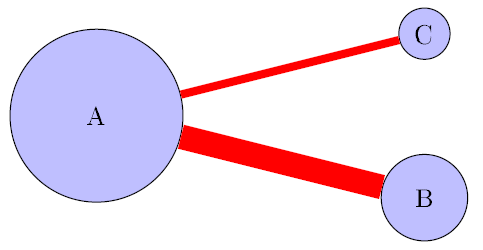
\includegraphics[width=0.3\linewidth]{grafo-ejemplo.png}
	\caption{Example of relationship between three people.}
	\label{fig:grafode2}
\end{figure}
%\vspace{-25pt}

This is, in the first instance, a characterization of the importance of individuals in the network.
However, more complex analytics could be applied.
%Esta es, en primera instancia, una caracterización de la importancia de los individuos en la red.
%Sin embargo, analíticas mas complejas podrían aplicarse.